166. \begin{figure}[ht!]
\center{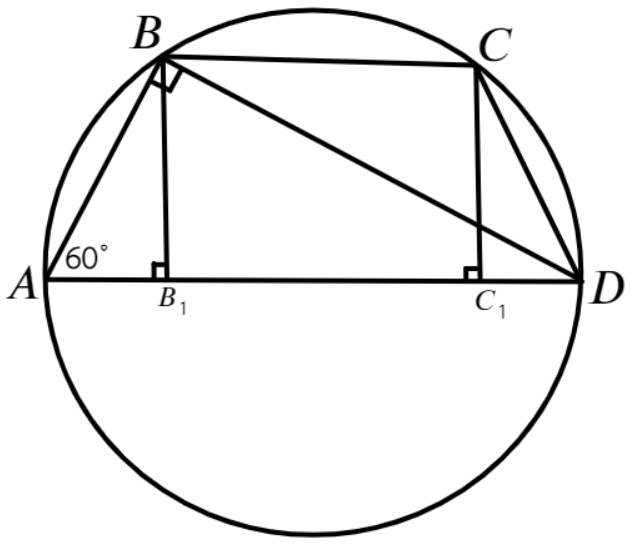
\includegraphics[scale=0.35]{g8-166.png}}
\end{figure}\\
а) Так как трапеция является вписанным четырёхугольником, $\angle A+\angle C=180^\circ.$ Но также $\angle A +\angle B=180^\circ,$ так как это односторонние углы, значит $\angle B=\angle C$ и трапеция является равнобокой.\\
б) Так как прямой угол опирается на диаметр, диаметром является $AD$ и $R=\cfrac{AD}{2}.$ Найдём $AB=CD=4,\ AD=AB:\cos(60^\circ)=4:\cfrac{1}{2}=8,$ тогда $R=8:2=4.$\\
в) Найдём $BD=AB\ tg(60^\circ)=4\cdot \sqrt{3}=4\sqrt{3}.$ Тогда $S_{\Delta ABD}=\cfrac{4\cdot4\sqrt{3}}{2}=8\sqrt{3}.$\\
г) Опустим высоты $BB_1$ и $CC_1,$ тогда $AB_1=C_1D=AB\cos(60^\circ)=4\cdot\cfrac{1}{2}=2,\ BC=B_1C_1=AD-AB_1-C_1D=8-2-2=4.$ Найдём высоту трапеции, она же равна высоте треугольника $BCD:\ BB_1=AB\sin(60^\circ)=4\cdot\cfrac{\sqrt{3}}{2}=2\sqrt{3},$ тогда $S_{\Delta BCD}=\cfrac{1}{2}\cdot2\sqrt{3}\cdot4=4\sqrt{3}.$\\
